\documentclass[handout]{beamer}
\usepackage[T1]{fontenc}
\usepackage[utf8]{inputenc}
\usepackage{lmodern}
\usepackage[italian]{babel}

\title{Il codice binario}
\author{\texorpdfstring{Mattia Cozzi\newline\href{mailto:cozzimattia@gmail.com}{\texttt{cozzimattia@gmail.com}}}{Mattia Cozzi}}
\date{a.s.~2023/2024}


%\documentclass[handout]{beamer}     %usare questa classe per generare l'handout

%\usepackage{pdfpages}   %per mostrare più quadri nella stessa pagina
%\pgfpagesuselayout{4 on 1}[a4paper,border shrink=5mm,landscape]


\usetheme{Singapore}
%\useoutertheme[left]{sidebar} %elementi intorno alle diapositive
\setbeamercovered{dynamic} %modifica l'aspetto del testo grigetto delle diapositive future. Argomenti: invisible/transparent/dynamic

%COLORE PRINCIPALE
\definecolor{verde}{RGB}{2, 194, 117} % UBC Blue (primary)
\setbeamercolor{structure}{fg=verde} % itemize, enumerate, etc
\setbeamercolor{alerted text}{fg=verde}


\usecolortheme{orchid}

\usepackage{tikz}
\usetikzlibrary{shapes.geometric, arrows}


\tikzstyle{startstop} = [ellipse, rounded corners, minimum width=3cm, minimum height=1cm,text centered, draw=black, fill=viola!30,text=white]
\tikzstyle{io} = [trapezium, trapezium left angle=70, trapezium right angle=110, minimum width=3cm, minimum height=1cm, text centered, draw=black, fill=viola!30,text=white]
\tikzstyle{process} = [rectangle, minimum width=3cm, minimum height=1cm, text centered, draw=black, fill=viola!30,text=white]
\tikzstyle{decision} = [diamond, minimum width=3cm, minimum height=1cm, aspect=2, text centered, draw=black, fill=viola!30,text=white]
\tikzstyle{arrow} = [thick,->,>=stealth]


\begin{document}

\begin{frame}
  \titlepage
\end{frame}


\begin{frame}
\frametitle{Contenuti}
\tableofcontents
\end{frame}

\section{Introduzione}

\begin{frame}
\frametitle{Definizioni}
\begin{block}{Computer}
  Il computer è una macchina elettronica capace di ricevere, trasmettere, memorizzare e soprattutto elaborare informazioni sotto forma di \emph{dati}.
\end{block}\pause

~

\begin{block}{Hardware}
  L'hardware è l'insieme delle parti elettroniche e meccaniche che compongono fisicamente il computer
\end{block}\pause

~

\begin{block}{Software}
  Il software è l'insieme delle parti immateriali a livello logico di un calcolatore (ad esempio un programma).
\end{block}
\end{frame}



\begin{frame}
\frametitle{Hardware (1)}
I componenti dell'hardware sono generalmente racchiusi dentro ad un \emph{case}{\pause} e sono, ad esempio:
\begin{columns}
  \begin{column}{0.4\textwidth}
    \begin{itemize}
      \item scheda madre;\pause
      \item CPU;\pause
      \item alimentatore elettrico;\pause
      \item memoria primaria (RAM);\pause
    \end{itemize}
    \end{column}
  \begin{column}{0.4\textwidth}
    \begin{itemize}
      \item memoria di massa;\pause
      \item scheda di rete;\pause
      \item scheda video;\pause
      \item scheda audio.
    \end{itemize}
    \end{column}
\end{columns}
\end{frame}



\begin{frame}
\frametitle{Hardware (2)}
\begin{figure}
  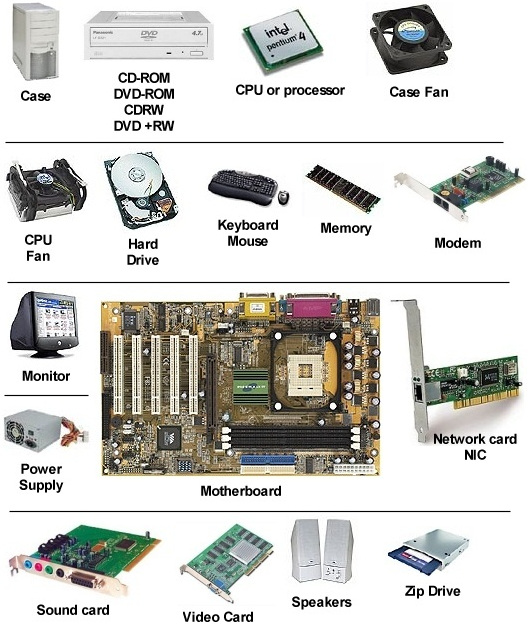
\includegraphics[width=.5\columnwidth]{img/hardware2.jpg}
\end{figure}
\end{frame}





\begin{frame}
\frametitle{Dati}
Un calcolatore riceve una serie di dati (sequenze di numeri e lettere) in ingresso, \alert<1>{esegue delle operazioni} su di essi e restituisce altri dati in uscita.\pause

~

I dati in ingresso sono chiamati in generale \alert<2>{input}.\pause

~

I dati in uscita sono chiamati invece \alert<3>{output}.
\end{frame}


\begin{frame}
\frametitle{Bit}
I dati che un calcolatore elettronico può trattare sono scritti nelle sue memorie (primaria e di massa) sotto forma di \alert<1>{bit}.\pause

~

La parola \emph{bit} nasce dall'unione di \emph{\textbf{bi}nary} e \emph{digi\textbf{t}}, cioè \alert<2>{cifra binaria}.\pause

~


\alert<3>{Una cifra binaria può valere 0 oppure 1}, mentre una cifra decimale può valere 0, 1, 2, 3, 4, 5, 6, 7, 8 oppure 9.\pause

~

A \alert<4>{livello fisico}, un bit può corrispondere a diversi stati: un interruttore alzato o abbassato, una corrente che può passare o meno, un campo magnetico orientato in un verso o nell'altro, etc.
\begin{center}
  \href{https://www.youtube.com/watch?v=zELAfmp3fXY}{\beamergotobutton{Bit con tavolette di legno}}
\end{center}
\end{frame}



\section{0 e 1}


\begin{frame}
\frametitle{Il sistema di numerazione decimale}
Il sistema di numerazione che utilizziamo abitualmente è un sistema decimale: ogni numero può essere scritto combinando le cifre da 0 a 9.\pause

~

La \alert<2>{posizione} di ogni cifra ne determina il valore.\pause

~

Sappiamo bene che 27 è ben diverso da 72: utilizzando le stesse cifre in ordine diverso otteniamo numeri differenti.
\end{frame}


\begin{frame}
\frametitle{Valore di una cifra e posizione}
Quando scriviamo il numero $ 5812 $ intendiamo dire:
\begin{center}
  5 migliaia, più 8 centinaia, più 1 decina, più 2 unità\pause
\end{center}
ovvero, in \alert<2>{notazione polinomiale}:
\begin{center}
  $ (5 \cdot 10^3) + (8 \cdot 10^2) + (1 \cdot 10^1) + (2 \cdot 10^0) $
\end{center}\pause

~

Vediamo come il valore di una cifra sia determinato da una \alert<3>{potenza di 10} (perché 10 sono le cifre che usiamo).\pause

~

\alert<4>{Attenzione:} si parte da $ 10^0 = 1 $.
\end{frame}



\begin{frame}
\frametitle{Il sistema di numerazione binario (1)}
Il sistema binario utilizza lo stesso procedimento, usando però \alert<1>{due sole cifre (0 e 1)} e di conseguenza le \alert<1-2>{potenze di 2}.\pause

~

\begin{center}
  $ 2^0=1 \qquad 2^1=2 \qquad 2^2=4 \qquad 2^3= 8 $

  ~

  $ 2^4=16 \qquad 2^5=32 \qquad 2^6=64 \qquad 2^7=128 $

  ~

  $ 2^8=256 \qquad 2^9=512 \qquad 2^{10}=1024 $

  ~

  \href{https://play2048.co/}{\beamergotobutton{Un gioco interessante}}
\end{center}
\end{frame}

\begin{frame}
\frametitle{Il sistema di numerazione binario (2)}
Esempi di numeri binari sono:

\begin{center}
  $ 101 \qquad\qquad 11101 \qquad\qquad 10001000 $
\end{center}\pause

~

Per convertirli in numerazione decimale basta lavorare come abbiamo fatto in precedenza per la numerazione decimale, \alert<2>{moltiplicando ogni cifra per la potenza di 2 corrispondente alla posizione occupata dalla cifra}.
\end{frame}

\begin{frame}
\frametitle{Conversione da binario a decimale (1)}
\begin{center}
  $ \alert<2>{1}\alert<3>{1}\alert<4>{0} $
\end{center}
Questo numero sarà convertito in numerazione decimale \alert<1>{utilizzando la scrittura polinomiale}:\pause
\begin{center}
  $ (\alert<2>{1} \cdot 2^2)\pause + (\alert<3>{1} \cdot 2^1)\pause + (\alert<4>{0} \cdot 2^0)\pause = 4 + 2 + 0 = 6 $
\end{center}\pause

~

Basterà sommare le potenze di 2 associate alla presenza della cifra 1 (perché $ 0 \cdot 2^n $ fa sempre 0).
\end{frame}


\begin{frame}
\frametitle{Conversione da binario a decimale (2)}
Convertiamo:
\begin{center}
  $ 111001 $
\end{center}\pause
Cominciamo da destra per iniziare comodamente con $ 2^0 $:
\begin{center}
  $ (1 \cdot 2^0)\pause + (1 \cdot 2^3)\pause + (1 \cdot 2^4)\pause + (1 \cdot 2^5)\pause = 1 + 8 + 16 + 32 = 57 $ 
\end{center}\pause

~

Prova a convertire:
\begin{center}
  $ 11111 \qquad \qquad 1000 \qquad \qquad 10001 $
\end{center}
\end{frame}


\begin{frame}
\frametitle{...}
\begin{quote}
  Al mondo ci sono 10 tipi di persone --{\pause} quelle che capiscono la numerazione binaria e quelle che non la capiscono.
\end{quote}\pause

~

~

\begin{quote}
  Al mondo ci sono 10 tipi di persone --{\pause} quelle che capiscono la numerazione ternaria, quelle che non la capiscono e quelle che la confondono con la numerazione binaria.
\end{quote}
\end{frame}



\begin{frame}
\frametitle{Conversione da decimale a binario (1)}
Per convertire un numero da decimale a binario si procede come segue:
\begin{itemize}
  \item si divide il numero per 2 (con resto 0 se è pari o 1 se è dispari);\pause
  \item si divide il quoziente ottenuto ancora per 2 (con resto 0 oppure 1);\pause
  \item si prosegue fino a ottenere quoziente zero;\pause
  \item si scrivono i resti, iniziando da sinistra con l'ultimo resto ottenuto.
\end{itemize}
\end{frame}

\begin{frame}
\frametitle{Conversione da decimale a binario (2)}
Ad esempio, per convertire il numero 159:

~

\begin{columns}
  \begin{column}{0.4\textwidth}
    $ 159 : 2 = 79 $, resto \alert<16>{$ 1 $}\pause

    ~

    $ 79 : 2 = 39 $, resto \alert<15>{$ 1 $}\pause

    ~

    $ 39 : 2 = 19 $, resto \alert<14>{$ 1 $}\pause


    ~

    $ 19 : 2 = 9 $, resto \alert<13>{$ 1 $}\pause
  \end{column}
  \begin{column}{0.4\textwidth}
    $ 9 : 2 = 4 $, resto \alert<12>{$ 1 $}\pause

    ~

    $ 4 : 2 = 2 $, resto \alert<11>{$ 0 $}\pause

    ~

    $ 2 : 2 = 1 $, resto \alert<10>{$ 0 $}\pause


    ~

    $ 1 : 2 = 0 $, resto \alert<9>{$ 1 $}\pause
  \end{column}
\end{columns}

~

~

Il numero 159, convertito in numerazione binaria, sarà quindi:
\begin{center}
  \alert<9>{1}\pause\alert<10>{0}\pause\alert<11>{0}\pause\alert<12>{1}\pause\alert<13>{1}\pause\alert<14>{1}\pause\alert<15>{1}\pause\alert<16>{1}
\end{center}
\end{frame}




\begin{frame}
\frametitle{Byte}
Un \emph{byte} è una sequenza di \alert<1>{8 bit}, cioè un numero binario costituito da 8 cifre.\pause

~

I valori minimo e massimo che un byte può assumere sono:
\begin{center}
  $ (00000000)_2 = (0)_{10} \qquad\qquad (11111111)_2 = (255)_{10} $
\end{center}\pause

~

Un byte può pertanto assumere $ 2^8 = 256 $ valori possibili.\pause

~

Il byte è l'unità di misura fondamentale della quantità di dati in informatica e i suoi multipli sono il kB, il MB, GB e TB (ognuno costituito da 1000 unità precedenti).
\end{frame}



\begin{frame}
\frametitle{Numerazione esadecimale (1)}
In informatica usiamo anche la numerazione esadecimale, che utilizza \alert<1>{sedici simboli}:
\begin{center}
  0, 1, 2, 3, 4, 5, 6, 7, 8, 9, A, B, C, D, E, F
\end{center}\pause
Le sei lettere che compaiono stanno ad indicare i numeri dopo il 9, cioè:
\begin{center}
  A = 10, B = 11, C = 12, D = 13, E = 14, F = 15
\end{center}
\end{frame}


\begin{frame}
\frametitle{Numerazione esadecimale (2)}
In numerazione esadecimale, con due simboli possiamo esprimere ben $ 16^2 = 256 $ numeri, con tre simboli ne possiamo esprimere $ 16^3 = 4096 $!\pause

~

Convertiamo ad esempio $ 2DF $:\pause
\begin{center}
  $ (2 \cdot 16^2) + (13 \cdot 16^1) + (15 \cdot 16^0) = $\pause

  ~

  $ = 512 + 208 + 15 = 735 $
\end{center}
\end{frame}

\section{Operazioni}

\begin{frame}
\frametitle{Calcolo binario}
Con in numeri scritti in numerazione binaria è possibile eseguire ovviamente le solite operazioni:\pause

~

\begin{itemize}
  \item addizione;\pause
  \item sottrazione;\pause
  \item moltiplicazione;\pause
  \item divisione.
\end{itemize}
\end{frame}



\begin{frame}
\frametitle{Addizione e sottrazione}
La somma segue lo stesso principio della somma decimale: si sommano le cifre corrispondenti dei due addendi, ricordando di ``riportare'' un 1 quando una somma tra cifre fa 2 o più.\pause

~

Calcoliamo $ 1010 + 1110 $:

\begin{table}[htp]\centering
  \begin{tabular}{rcccccc}\rule{0pt}{3ex}
    \visible<4->{riporto}    & \visible<6->{\alert<6>{1}} & \visible<5->{\alert<5>{1}} & \visible<4->{\alert<4>{1}} &   &   &   \\\rule{0pt}{3ex}
        I addendo  &   & 1 & 0 & 1 & 0 & + \\\rule{0pt}{3ex}
        II addendo &   & 1 & 1 & 1 & 0 & = \\\hline\rule{0pt}{3ex}
        risultato  & \visible<7->{1} & \visible<6->{1} & \visible<5->{0} & \visible<4->{0} & \visible<3->{0} &  \\
  \end{tabular}
\end{table}

~

\visible<8>{In modo analogo possiamo eseguire la differenza, ricordando che invece del ``riporto'' dovremo usare dei ``prestiti''.}
\end{frame}


\begin{frame}
\frametitle{Moltiplicazione}
Anche la moltiplicazione segue le solite regole, ricordando ancora che 2 unità di un certo ordine equivalgono ad 1 unità dell'ordine superiore (così come 10 centinaia fanno 1 migliaio).\pause

~

Eseguiamo $ 110 \times 101 $:
\begin{table}[htp]\centering
  \begin{tabular}{rcccccc}\rule{0pt}{3ex}
        I fattore             &   &   & \alert<3-5>{1} & \alert<3-5>{1} & \alert<3-5>{0} & $\times$ \\\rule{0pt}{3ex}
        II fattore            &   &   & \alert<5>{1} & \alert<4>{0} & \alert<3>{1} & = \\\hline\rule{0pt}{3ex}\pause
        I prodotto parziale   &   &   & \alert<3>{1} & \alert<3>{1} & \alert<3>{0} &  \\\rule{0pt}{3ex}\pause
        II prodotto parziale  &   & \alert<4>{0} & \alert<4>{0} & \alert<4>{0} & - &  \\\rule{0pt}{3ex}\pause
        III prodotto parziale & \alert<5>{1} & \alert<5>{1} & \alert<5>{0} & - & - &  \\\hline\rule{0pt}{3ex}\pause
        risultato             & 1 & 1 & 1 & 1 & 0 &  \\
  \end{tabular}
\end{table}
\end{frame}



\begin{frame}
\frametitle{Le operazioni logiche}
Con i numeri binari possiamo anche eseguire operazioni particolari dette \alert<1>{operazioni logiche o booleane} (dal nome del logico del XIX secolo George Boole).\pause

~

Le operazioni logiche più comuni sono:
\begin{itemize}
  \item \alert<2>{AND} (congiunzione), indicata anche con $\& $ oppure $\wedge$;\pause
  \item \alert<3>{OR} (disgiunzione), indicata anche con $\vee $;\pause
  \item \alert<4>{NOT} (negazione).\pause
\end{itemize}

~

Se consideriamo la cifra 0 come valore di verità ``falso'' e la cifra 1 come ``vero'', possiamo comprendere meglio il senso delle operazioni logiche.
\end{frame}



\begin{frame}
\frametitle{NOT}
Corrisponde alla negazione e tramuta uno 0 in un 1 e viceversa.

~

\begin{table}[htp]\centering
  \begin{tabular}{c|c}\rule{0pt}{3ex}
         \textbf{X} & \textbf{NOT(X)}  \\\hline\rule{0pt}{3ex}
         0 & 1 \\\hline\rule{0pt}{3ex}
         1 & 0 \\
  \end{tabular}
\end{table}\pause

~


~

È un operatore unario perché riceve in ingresso un solo numero (bit).
\end{frame}


\begin{frame}
\frametitle{Esempio}
\begin{table}[htp]\centering
  \begin{tabular}{ccccc}\rule{0pt}{3ex}
         \textbf{X}      & 1 & 0 & 1 & 1 \\\rule{0pt}{3ex}\pause
                         & $ \visible<2>{\downarrow} $ & $ \visible<3>{\downarrow} $ & $ \visible<4>{\downarrow} $ & $ \visible<5>{\downarrow} $ \\\rule{0pt}{3ex}
         \textbf{NOT(X)} & \visible<2->{0} & \visible<3->{1} & \visible<4->{0} & \visible<5->{0} \\
  \end{tabular}
\end{table}
\end{frame}



\begin{frame}
\frametitle{AND}
Corrisponde alla congiunzione e restituisce un 1 solo se entrambi i bit in ingresso valgono 1.

~

\begin{table}[htp]\centering
  \begin{tabular}{c|c|c}\rule{0pt}{3ex}
         \textbf{X} & \textbf{Y} & \textbf{X AND Y}  \\\hline\rule{0pt}{3ex}
         1 & 1 & 1 \\\hline\rule{0pt}{3ex}
         1 & 0 & 0 \\\hline\rule{0pt}{3ex}
         0 & 1 & 0 \\\hline\rule{0pt}{3ex}
         0 & 0 & 0 \\
  \end{tabular}
\end{table}

~


~

È un operatore binario perché riceve in ingresso due bit.
\end{frame}


\begin{frame}
\frametitle{Esempio}
\begin{table}[htp]\centering
  \begin{tabular}{ccccc}\rule{0pt}{3ex}
         \textbf{X}      & 1 & 0 & 0 & 1 \\\rule{0pt}{3ex}
         \textbf{Y}      & 1 & 1 & 0 & 1 \\\rule{0pt}{3ex}\pause
                         & $ \visible<2>{\downarrow} $ & $ \visible<3>{\downarrow} $ & $ \visible<4>{\downarrow} $ & $ \visible<5>{\downarrow} $ \\\rule{0pt}{3ex}
         \textbf{X AND Y} & \visible<2->{1} & \visible<3->{0} & \visible<4->{0} & \visible<5->{1} \\
  \end{tabular}
\end{table}
\end{frame}



\begin{frame}
\frametitle{OR}
Corrisponde alla disgiunzione e restituisce un 1 se almeno uno dei due bit in ingresso vale 1.

~

\begin{table}[htp]\centering
  \begin{tabular}{c|c|c}\rule{0pt}{3ex}
         \textbf{X} & \textbf{Y} & \textbf{X OR Y}  \\\hline\rule{0pt}{3ex}
         1 & 1 & 1 \\\hline\rule{0pt}{3ex}
         1 & 0 & 1 \\\hline\rule{0pt}{3ex}
         0 & 1 & 1 \\\hline\rule{0pt}{3ex}
         0 & 0 & 0 \\
  \end{tabular}
\end{table}

~


~

È un operatore binario perché riceve in ingresso due bit.
\end{frame}





\begin{frame}
\frametitle{Esempio}
\begin{table}[htp]\centering
  \begin{tabular}{ccccc}\rule{0pt}{3ex}
         \textbf{X}      & 1 & 0 & 0 & 1 \\\rule{0pt}{3ex}
         \textbf{Y}      & 1 & 1 & 0 & 1 \\\rule{0pt}{3ex}\pause
                         & $ \visible<2>{\downarrow} $ & $ \visible<3>{\downarrow} $ & $ \visible<4>{\downarrow} $ & $ \visible<5>{\downarrow} $ \\\rule{0pt}{3ex}
         \textbf{X OR Y} & \visible<2->{1} & \visible<3->{1} & \visible<4->{0} & \visible<5->{1} \\
  \end{tabular}
\end{table}
\end{frame}

%%% SISTEMA ESADECIMALE!!!! https://www.lezionidimatematica.net/Binario/lezioni/bin_lezione_12.htm


\section{Scrittura binaria}


\begin{frame}
\frametitle{Codificare un'informazione (1)}
Codificare un'informazione significa tradurre un certo dato in uno specifico codice, nel nostro caso \alert<1>{codice binario}.\pause

~

Per esempio, se vogliamo codificare $ 16 = 2^4 $ simboli (15 lettere e uno spazio vuoto) ci serviranno 4 bit:
\begin{table}[htp]\centering
  \begin{tabular}{|c|c|}\hline\rule{0pt}{3ex}
    A & 0000 \\\hline\rule{0pt}{3ex}
    B & 0001 \\\hline\rule{0pt}{3ex}
    C & 0010 \\\hline\rule{0pt}{3ex}
    D & 0011 \\\hline
  \end{tabular}~~~~
  \begin{tabular}{|c|c|}\hline\rule{0pt}{3ex}
    E & 0100 \\\hline\rule{0pt}{3ex}
    F & 0101 \\\hline\rule{0pt}{3ex}
    G & 0110 \\\hline\rule{0pt}{3ex}
    H & 0111 \\\hline
  \end{tabular}~~~~
  \begin{tabular}{|c|c|}\hline\rule{0pt}{3ex}
    I & 1000 \\\hline\rule{0pt}{3ex}
    L & 1001 \\\hline\rule{0pt}{3ex}
    M & 1010 \\\hline\rule{0pt}{3ex}
    N & 1011 \\\hline
  \end{tabular}~~~~
  \begin{tabular}{|c|c|}\hline\rule{0pt}{3ex}
    O & 1100 \\\hline\rule{0pt}{3ex}
    P & 1101 \\\hline\rule{0pt}{3ex}
    Q & 1110 \\\hline\rule{0pt}{3ex}
    \textvisiblespace & 1111 \\\hline
  \end{tabular}
  \end{table}
\end{frame}



\begin{frame}
\frametitle{Codificare un'informazione (2)}
Prova, con la codifica precedente, a \alert<1-2>{decodificare} questo messaggio:
\begin{center}
  $ 0000 1001 1000 1111 0011 1000 1111 1101 1100 1001 1001 1100 $
\end{center}

~

Ci rendiamo subito conto che è possibile decodificare un messaggio solo se ogni simbolo è \alert{rappresentato dallo stesso numero di bit} (non sapremmo infatti dire altrimenti dove finisce e dove inizia un nuovo simbolo).\pause

~

Lo ``spazio'' occupato dipende ovviamente dalla lunghezza del messaggio e dal tipo di codifica.
\end{frame}


\begin{frame}
\frametitle{Esempio}
Prova, con la codifica precedente, a \alert{decodificare} questo messaggio:
\begin{center}
  
\end{center}
\end{frame}


\begin{frame}
\frametitle{La tabella ASCII (1)}
Il codice ASCII fu inventato molti anni fa per le comunicazioni fra telescriventi, per poi diventare uno \alert<1>{standard mondiale}.\pause

~

ASCII sta per ``American Standard Code for Information Interchange'', ovvero ``Standard americano per lo scambio di informazioni''.\pause

~

Mediante questa codifica era possibile far riferimento ad un carattere di testo mediante un numero binario a 7 bit, fino ad un massimo di $2^7 = 128 $ caratteri.

~

Ad esempio il carattere ``\texttt{@}'' è rappresentato dal codice ASCII ``64'', ``Y'' dall'``89'', ecc.
\end{frame}

\begin{frame}
  \frametitle{La tabella ASCII (2)}
\begin{columns}
\begin{column}{.33\textwidth}
  \begin{center}
    \begin{figure}
      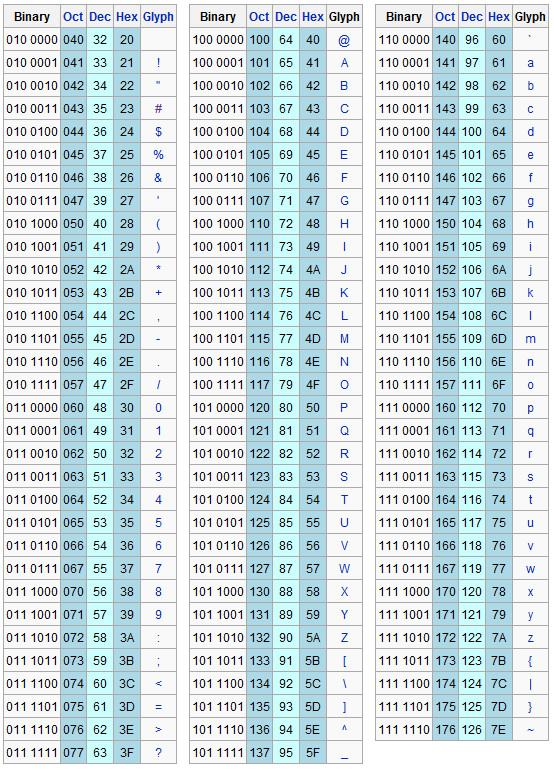
\includegraphics[width=\columnwidth]{img/ascii1.jpg}
    \end{figure}
  \end{center}
\end{column}
\begin{column}{.33\textwidth}
  \begin{center}
    \begin{figure}
      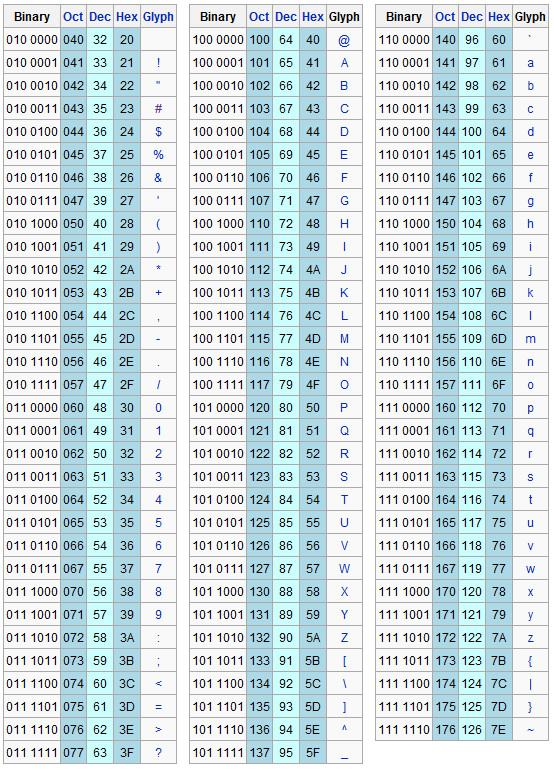
\includegraphics[width=\columnwidth]{img/ascii2.jpg}
    \end{figure}
  \end{center}
\end{column}
\begin{column}{.33\textwidth}
  \begin{center}
    \begin{figure}
      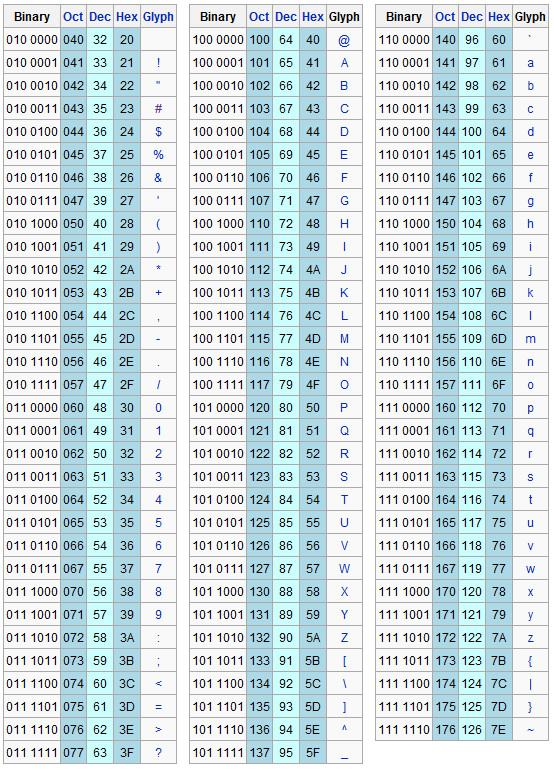
\includegraphics[width=\columnwidth]{img/ascii3.jpg}
    \end{figure}
  \end{center}
\end{column}
\end{columns}
\end{frame}


\begin{frame}
\frametitle{Altre codifiche}
La tabella ASCII è stata poi estesa in vari modi utilizzando l'ottavo bit disponibile di un byte.\pause

~

Lo standard per la codifica del testo attualmente utilizzato è \alert<2>{UNICODE}, compatibile con ASCII.\pause

~

Ad oggi UNICODE conta circa 150.000 caratteri codificati, comprendendo anche lingue antiche, simboli ed emoji.
\end{frame}

\begin{frame}
\frametitle{La codifica delle immagini}
Un'immagine su uno schermo è costituita da un insieme di pixel affiancati, ognuno con uno specifico colore.
\begin{figure}
  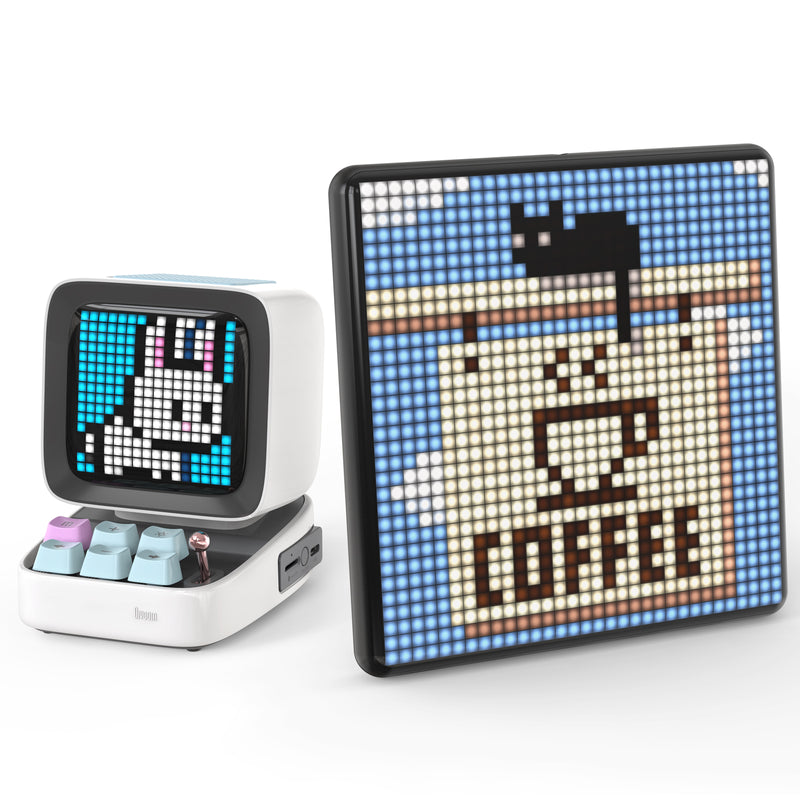
\includegraphics[width=.3\columnwidth]{img/pixel.jpg}
\end{figure}\pause
Per digitalizzarla (trasformarla in una sequenza di 0 e 1) possiamo memorizzare il colore di ogni singolo pixel.\pause

~

Questo metodo tuttavia non è molto efficiente: molti dati si ripetono uguali.
\end{frame}


\begin{frame}
\frametitle{La \emph{palette di colori}}
\begin{columns}
\begin{column}{.3\textwidth}
  \begin{figure}
    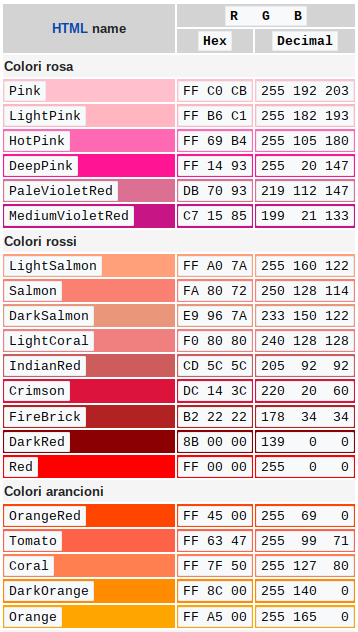
\includegraphics[width=\columnwidth]{img/palette.png}

    \small{Palette di colori X11}
  \end{figure}
\end{column}
\begin{column}{.5\textwidth}
  Un'altra opzione è creare una tavolozza di colori (\emph{palette}), per poi dare il colore di ogni singolo pixel in riferimento alla \emph{palette}.\pause

  ~

  Questo metodo è utile per immagini di grandi dimensioni, in cui lo spazio utilizzato per memorizzare la \emph{palette} è ampiamente ripagato dal risparmio di dati sull'intera immagine.
\end{column}
\end{columns}
\end{frame}


\begin{frame}
\frametitle{Codice alfanumerico}
Un codice alfanumerico è una stringa costituita soltanto da numeri e lettere (maiuscole o minuscole).\pause

~

Se per il codice ASCII servono 8 bit, cioè 1 byte, per un codice alfanumerico ne bastano 6.\pause

~

Infatti, considerando le lettere maiuscole e minuscole (26 + 26) e i numeri (10), si ottiene un numero totale di simboli minore di $ 2^6 = 64 $.
\end{frame}






\end{document}
